%%%%quick build setup user setting for  knitr + pytex
%%  here->    r -e "knitr::knit('%.Rnw')"|pdflatex -synctex=1 -interaction=nonstopmode %.tex|pythontex %.pytexcode|pdflatex -synctex=1 -interaction=nonstopmode %.tex|"C:/Program Files/Adobe/Reader 11.0/Reader/AcroRd32.exe" %.pdf

%%%%quick build setup user setting for only knitr
%%  here->    r -e "knitr::knit('%.Rnw')"|pdflatex -synctex=1 -interaction=nonstopmode %.tex|"C:/Program Files/Adobe/Reader 11.0/Reader/AcroRd32.exe" %.pdf

%%%%quick build setup user setting for only pytex
%%  here->    pdflatex -synctex=1 -interaction=nonstopmode %.tex|pythontex %.pytexcode|pdflatex -synctex=1 -interaction=nonstopmode %.tex|"C:/Program Files/Adobe/Reader 11.0/Reader/AcroRd32.exe" %.pdf



\documentclass{article}\usepackage[]{graphicx}\usepackage[]{color}
% maxwidth is the original width if it is less than linewidth
% otherwise use linewidth (to make sure the graphics do not exceed the margin)
\makeatletter
\def\maxwidth{ %
  \ifdim\Gin@nat@width>\linewidth
    \linewidth
  \else
    \Gin@nat@width
  \fi
}
\makeatother

\definecolor{fgcolor}{rgb}{0.345, 0.345, 0.345}
\newcommand{\hlnum}[1]{\textcolor[rgb]{0.686,0.059,0.569}{#1}}%
\newcommand{\hlstr}[1]{\textcolor[rgb]{0.192,0.494,0.8}{#1}}%
\newcommand{\hlcom}[1]{\textcolor[rgb]{0.678,0.584,0.686}{\textit{#1}}}%
\newcommand{\hlopt}[1]{\textcolor[rgb]{0,0,0}{#1}}%
\newcommand{\hlstd}[1]{\textcolor[rgb]{0.345,0.345,0.345}{#1}}%
\newcommand{\hlkwa}[1]{\textcolor[rgb]{0.161,0.373,0.58}{\textbf{#1}}}%
\newcommand{\hlkwb}[1]{\textcolor[rgb]{0.69,0.353,0.396}{#1}}%
\newcommand{\hlkwc}[1]{\textcolor[rgb]{0.333,0.667,0.333}{#1}}%
\newcommand{\hlkwd}[1]{\textcolor[rgb]{0.737,0.353,0.396}{\textbf{#1}}}%
\let\hlipl\hlkwb

\usepackage{framed}
\makeatletter
\newenvironment{kframe}{%
 \def\at@end@of@kframe{}%
 \ifinner\ifhmode%
  \def\at@end@of@kframe{\end{minipage}}%
  \begin{minipage}{\columnwidth}%
 \fi\fi%
 \def\FrameCommand##1{\hskip\@totalleftmargin \hskip-\fboxsep
 \colorbox{shadecolor}{##1}\hskip-\fboxsep
     % There is no \\@totalrightmargin, so:
     \hskip-\linewidth \hskip-\@totalleftmargin \hskip\columnwidth}%
 \MakeFramed {\advance\hsize-\width
   \@totalleftmargin\z@ \linewidth\hsize
   \@setminipage}}%
 {\par\unskip\endMakeFramed%
 \at@end@of@kframe}
\makeatother

\definecolor{shadecolor}{rgb}{.97, .97, .97}
\definecolor{messagecolor}{rgb}{0, 0, 0}
\definecolor{warningcolor}{rgb}{1, 0, 1}
\definecolor{errorcolor}{rgb}{1, 0, 0}
\newenvironment{knitrout}{}{} % an empty environment to be redefined in TeX

\usepackage{alltt}



\input{C:/Users/ajh01/Desktop/Folder/oldtex/hdr/hdrk}
\usepackage{verbatim}
\usepackage{fullpage}
\usepackage{wrapfig}
\usepackage{float}
\usepackage{transparent}
\usepackage{pstricks}


\addtolength{\oddsidemargin}{.05in}
\addtolength{\topmargin}{-.50in}
\addtolength{\textheight}{1in}
\reversemarginpar
\addtolength{\headsep}{.25in}
\parskip = 5pt plus 0pt minus 0pt
\pagestyle{myheadings}
\setlength{\parindent}{0in}



\newcommand{\pd}{\frac{\partial }{\partial \dot{q}}}
\newcommand{\Rn}{\mathbb{R}^n}
\newcommand{\M}{\mathcal{M}}

%%%%%%%%%%%%%%%%%%%%%%%%%


\title{Variational Mechanics}%%Title
\author{Alexander J. Heilman}%%Name
\date{revised: \today}%%Date
\markright{Variational Mechanics}%%Heading



%%%%%%%%%%%%%%%%%%%%%%%%%

\IfFileExists{upquote.sty}{\usepackage{upquote}}{}
\begin{document}

\maketitle


\tableofcontents

\pagebreak

\section*{Literature Review}

V.I. Arnold


Jessica Coopersmith's \textit{The Lazy Universe} \cite{coopersmith} gives the most philosophically motivated (if not just lengthy) development of the principle of stationary action from the principle of virtual work (derives form of L). However, it lacks the more modern mathematical machinery of variational mechanics.

Cornelius Lanczos' \textit{The Variational Principles of Mechanics} \cite{lanczos} is a classic introduction and relatively in-depth development of variational mechanics from the principle of virtual work (derives form of L). Good for guided mathematical development aswell as concurrent and independent philosophical considerations.

Landau and Lifshitz' first volume of several hefty physics textbooks \textit{Course in Theoretical Physics} \cite{landau} takes the principle of stationary action as a given but develops the beginnings of variational mechanics from there.

David Cline's \textit{Variational Principles in Classical Mechanics} \cite{cline} gives good exposition on the topic.

Goldstein, Poole, and Safko's \textit{Analytical Mechanics} \cite{goldstein} gives a brief development of D'Alembert's Principle and then independently considers Hamilton's Principle and the basic tools of variational mechanics. However, some may not be able to bear looking at the book for too long.


Davidson Soper's \textit{Classical Field Theory} \cite{soper} gives a development of variational mechanics in field theory from the particle paradigm.

\section{Assumptions/Intro}

This short and informal document gives a brief (and mathematically incomplete) derivation of the E-L equations, building essentially from D'Alembert's principal to Hamilton's principle. It is intended to give a somewhat concise statement of the simplest form of these principles and equations to aid in physical and philosophical considerations relevant thereto.

These principles are given in their simplest form, as mentioned above, given they are relevant to systems concerning only particles (as opposed to fields) and classical forces (as opposed to quantum or relativistic). Generally we will also assume the Lagrangian's dependence on time is only contributed through the path $q(t)$ and it's velocity $\dot{q}(t)$, and will denote this with the standard notation $\frac{\partial L}{\partial t}=0$. We will further assume that the path taken, and its first derivative with respect to time, is continuous. 

Further, D'Alembert's principle here still implies the adoption of the Newtonian relation that forces correspond to a change in momentum , i.e. $I=\frac{dp}{dt}$. And we will also assume applied forces to be the differential of some corresponding scalar function, $F=-\frac{dV}{dr}$.


%%\section{Newtonian Relation}


%%\section{Principle of Virtual Work}


\section{D'Alembert's Principle}

The principle of virtual work for static equilibrium ($\sum_i{F_i\cdot \delta \vec{\textbf{r}}_i}=0$) can be adapted to dynamical systems by treating the reactions of massive bodies as 'inertial forces' exactly balancing imparted forces. This adapted principle can be described as below,

\begin{equation}
\textit{D'Alembert's Principle:} \quad \sum_{i}{(F_{i}-I_{i})\cdot\delta \vec{\textbf{r}}_{i}}=0 
\end{equation}

where $F_i=F^{Applied}_i+f^{constraint}_{i}$ is the sum of applied and constraint forces on object $i$; $I_i=\frac{d}{dt}(m\vec{v})$ is the modeled inertial force for object $i$; and $\delta \vec{\textbf{r}}$ is the virtual displacement (virtual stipulating it occurs not over time but in some instant, so as to prevent conditions from changing). Assuming displacements happen "harmoniously" with respect to the constraints, i.e. the constraints are satisfied perfectly, the term in $F_i$ accounting for constraints can generally be omitted from considerations as it disappears independently with $\sum_i{f^{constraint}_i}\cdot\delta\vec{\textbf{r}}=0$. Further, since conservative forces can be modeled as the differential of a scalar field, $-\frac{dV}{d\vec{r}}=F$, the first term can be considered a direct variation in a suitable potential energy, $\delta V$.

\begin{center}
$\sum_{i}{(F_{i})\cdot\delta \vec{\textbf{r}}_{i}}=\sum_{i}{(-\frac{dV}{d\vec{r}})\cdot\delta \vec{\textbf{r}}_{i}}=\sum_{i}{-\delta V_i}$
\end{center}

where the summation is still over $i$ particles. We neglect to generalize coordinates and forces here as it is accomplished with a simple application of the chain rule.

\section{Hamilton's Principle}

A logically equivalent principle to D'Alembert's principle that is extensible to dynamical systems over a given time or path is Hamilton's principle. It may be considered as the minimization of an integral over some virtual displacement in path $\delta\vec{\textbf{r}}$, where the variation (and it's derivative) is continuous and vanishes at the points denoted by $t_a$ and $t_b$.

\begin{equation}
\textit{Hamilton's Principle:} \quad\int_{t_a}^{t_b}dt \sum_{i}{(F_{i}-I_{i})\cdot\delta \vec{\textbf{r}}_{i}}=0
\end{equation}

The second term here, $I_i\cdot\delta \vec{\textbf{r}}$, can be expanded as $\frac{d}{dt}(m\vec{v})\cdot\delta \vec{\textbf{r}}$ and by the product rule, we know $\frac{d}{dt}(m\vec{v}\cdot \delta \vec{\textbf{r}})=\frac{d}{dt}(m\vec{v})\cdot \delta\vec{\textbf{r}}+m\vec{v}\cdot\delta\vec{\textbf{v}}$.

\begin{center}

$\int_{t_a}^{t_b}dt\left[\frac{d}{dt}(m\vec{v})\cdot\delta \vec{\textbf{r}}\right]
=\int_{t_a}^{t_b}dt\left[ \frac{d}{dt}(m\vec{v}\cdot \delta \vec{\textbf{r}})-m\vec{v}\cdot\delta\vec{\textbf{v}}\right]
=[m\vec{v}\cdot \delta \vec{\textbf{r}}]\vert_{t_a}^{t_b}-\int_{t_a}^{t_b}dt[m\vec{v}\cdot\delta\vec{\textbf{v}}]$

\end{center}

Recalling the property of $\delta\vec{\textbf{r}}$ that requires it vanish at the boundaries $t_a$ and $t_b$, it follows that any dot product with it at those points vanishes as well so the first term here is zero. We can also develop $\int_{t_a}^{t_b}dt[m\vec{v}\cdot\delta\vec{\textbf{v}}]$ into a variation of a scalar function of $\vec{v}$ (namely a function of $v^2$) as follows. 

\begin{center}

$-\int_{t_a}^{t_b}[m\vec{v}\cdot\delta\vec{\textbf{v}}]dt=-\int_{t_a}^{t_b}\delta\left[ \frac{m}{2}\vec{v}\cdot\vec{v}\right] dt
=-\delta\int_{t_a}^{t_b}Tdt$

\end{center}

The scalar function $T=\frac{1}{2}mv^2$ is defined as the kinetic energy of the particle. Here we have neglected the summation term due to the linearity of the integral. Thus, Hamilton's principle can be simplified as such,

\begin{equation}
\delta\int_{t_a}^{t_b}(T-V)dt=0
\end{equation}

and we may further define the quantity $T-V$ as the Lagrangian $L=T-V$.

\section{Euler-Lagrange Equations}

In this context, we'd like to minimize the variation of a functional in the following form.

\begin{equation}
\delta\int^{t_b}_{t_a}L(\vec{q},\dot{\vec{q}})dt 
\end{equation}   

\begin{center}

\begin{figure}
\input{qtform.pdf_tex}
\caption{Some minimal path $q(t)$ and deviations (Note the fixed endpoints)}
\end{figure}

\end{center}

Where $L=T-V$ is a function of a path through some generalized coordinates, $q$; and their derivatives with respect to time $\dot{q}$. The path in this context is parameterized by time, and can be considered to really be what is being varied. We stipulate that it and it's time derivative be continuous. As such, $q$ could have the form:

\begin{center}
$q(t,\epsilon)=Q(t)+\epsilon\eta(t)$

$\dot{q}(t,\epsilon)=\dot{Q}(t)+\epsilon\dot{\eta}(t)$


\end{center}

where $Q(t)$ is the path that minimizes the functional; and $\epsilon\eta(t)$ is any allowable variation in path (one that is continuous and vanishing at endpoints),$\eta(t)$, multiplied by a free scalar, $\epsilon$. We are free to multiply the variation in path here by an arbitrary scalar of our choosing as any path that is continuous and vanishes at certain points clearly satisfies those same properties when multiplied by a scalar. In this form, we may consider the previous integral as:

\begin{equation}
\delta\int^{t_b}_{t_a}L(\vec{q},\dot{\vec{q}})dt=\frac{d}{d\epsilon}\int^{t_b}_{t_a}L(\vec{q},\dot{\vec{q}})dt=\int^{t_b}_{t_a}\left( \frac{dL}{dq}\frac{dq}{d\epsilon}+\frac{dL}{d\dot{q}}\frac{d\dot{q}}{d\epsilon}\right) dt=0
\end{equation}

Considering the prior given form of $q$, we have $\frac{dq}{d\epsilon}=\eta(t)$ and $\frac{d\dot{q}}{d\epsilon}=\dot{\eta}(t)$. Further, integration by parts will allow us to convert the second term in the expansion to a product with $\eta(t)$ instead, as follows



$$\int\frac{d}{dt}\left( \frac{dL}{d\dot{q}}\frac{dq}{d\epsilon} \right) dt
=\int\left(\frac{d}{dt}\left(\frac{dL}{d\dot{q}}\right)\frac{dq}{d\epsilon}+\frac{dL}{d\dot{q}}\frac{d\dot{q}}{d\epsilon}\right)dt=\left( \frac{dL}{d\dot{q}}\eta \right) \vert^{t_b}_{t_a}=0
$$
 
Where once again, the total differential integrates to zero given the vanishing boundary conditions. This gives us the equality,

$$
\frac{d}{dt}\left(\frac{dL}{d\dot{q}}\right)\frac{dq}{d\epsilon}=-\frac{dL}{d\dot{q}}\frac{d\dot{q}}{d\epsilon}
$$

Substituting in $\frac{dq}{d\epsilon}=\eta$ and the above equality into the expanded variation now gives

\begin{equation}
\int^{t_b}_{t_a}\left( \frac{dL}{dq}\frac{dq}{d\epsilon}+\frac{dL}{d\dot{q}}\frac{d\dot{q}}{d\epsilon}\right) dt=\int^{t_b}_{t_a}\left[ \frac{dL}{dq} -\frac{d}{dt}\left( \frac{dL}{d\dot{q}}\right)  \right] \eta(t) \ dt=0
\end{equation}

And given that this is satisfied for any variation, $\eta(t)$, from the minimizing path $Q$, it follows that the quantity in the brackets must vanish for the minimizing path.




\section{Lagrangian on a Manifold}
Given the tangent bundle $T\mathcal{M}$ of some differentiable configuration manifold $\mathcal{M}$, the Lagrangian $L$ can be defined as a function from the tangent bundle to the real numbers, i.e. $L:T\mathcal{M}\rightarrow\mathbb{R}$. A motion $\gamma$ in the Lagrangian system given above is then a curve $\mathbb{R}\rightarrow\mathcal{M}$ extremal of the functional $\Phi[\gamma]=\int L(\gamma ,\gamma')dt$, where $\gamma'\in T\mathcal{M}$.

\input{drawingr4.pdf_tex}


\pagebreak


%%\begin{figure}
%%\input{drawing.pdf_tex}
%%\caption{Parametrized Integration by Parts}
%%\end{figure}

\section{Conjugate Coordinates}

Now, let's define

\begin{equation}
p=\frac{\partial L}{\partial \dot{q}}.
\end{equation}



This is a coordinate conjugate to $q$ in that it replaces the dependence on $\dot{q}$ in the Legendre transform of $L$ (which is $H$). 

$$
\frac{\partial }{\partial \dot{q}}H=\pd\left( p\dot{q} \right)-\pd L
$$

\section{Construction of Hamiltonian}

The Hamiltonian is the Legendre transform of the Lagrangian, and reduces the problem of solving the second order E-L eqs. into a pair of coupled first order equations. It's effective for qualitative analysis of larger scale behaviour of systems, and is particularly suited for investigation of conserved quantities.



Considering the explicit time dependence of the function 
$L=T-V$ here is zero, we can derive that $L$'s dependence on time is due to the following contributions

$$
\frac{d}{dt}L(q,\dot{q})=
\frac{dL}{dq}\frac{dq}{dt}+
\frac{dL}{d\dot{q}}\frac{d\dot{q}}{dt}=
\frac{dL}{dq}\dot{q}+
\frac{dL}{d\dot{q}}\ddot{q}
$$

Now assuming we're traveling along the minimizing path satisfying the E-L eqs., $\frac{d}{dt}\left( \frac{dL}{d\dot{q}}\right) =\frac{dL}{dq}$, and the relation $\frac{d}{dt}\left( \frac{dL}{d\dot{q}}\dot{q}\right) =\frac{d}{dt}\left( \frac{dL}{d\dot{q}} \right) \dot{q}+\frac{dL}{d\dot{q}}\ddot{q}$

$$
\frac{d}{dt}L(q,\dot{q})=\frac{d}{dt}\left( \frac{dL}{d\dot{q}} \right) \dot{q}+\frac{dL}{d\dot{q}}\ddot{q}=\frac{d}{dt}
\left( \frac{dL}{d\dot{q}}\dot{q}\right)
$$

Combining terms on one side gives us

\begin{equation}
\frac{d}{dt}
\left( \frac{dL}{d\dot{q}}\dot{q}-L\right)=0
\end{equation}

Where we label the term being differentiated $E$, the energy of the system. $E$ is equivalent to $H$, but the rebranding emphasizes a change in input coordinates as $E$ is still specified in terms of paths through $q$ and $\dot{q}$; but $H$ is specified in paths through $q$ and $p=\frac{\partial L}{\partial \dot{q}}$. 


\section{Noether's Theorem}


$$
\int dt\wedge dr \left( 
-\frac{dU}{dr}+\frac{dp}{dt}
 \right)
$$


Noether's theorem formalizes the correspondence between symmetries of the Lagrangian and conserved quantities of the minimal path.








%\begin{wrapfigure}{r}{.6\textwidth}
\vspace{7cm}
  \begin{center}
    \begin{figure}
   \input{drawing.pdf_tex}
 
 \vspace{-1cm}

\caption{Parametrized Integration by Parts}

  
\end{figure}  
   \end{center}
 % \vspace{0pt}
%\end{wrapfigure}


%\begin{wrapfigure}{r}{.6\textwidth}
  \begin{center}


   \end{center}
 % \vspace{0pt}
%\end{wrapfigure}

\pagebreak

\section{Symplectic Notes}

The following notes follow Tobias Osbourne's lectures on Symplectic Geometry and Classical Mechanics %ref%.

\textbf{Definition:} A \textit{locally Euclidean space} $\mathcal{M}$ of dimension $d$ is a Hausdorff topological space for which every point $p\in \mathcal{M}$ has a neighborhood homeomorphic to an open subset of $\mathbb{R}^d$.


%\includegraphics[scale=.65]{drawing.eps}

\input{drawingt.pdf_tex}

\textbf{Definition:} A \textit{differentiable structure} $\mathcal{F}$ of class $C^k\ (1\leq k \leq \inf)$ on a locally Euclidean space $\mathcal{M}$ is a collection of charts $\lbrace (U_x , \phi_x)\vert \alpha \in A \rbrace$ satisfying 

(i) $\bigcup_{\alpha \in A}=\mathcal{M}$

(ii) $\phi_{\alpha}\circ\phi_{\beta}^{-1}$ is $C^k$ for all $\alpha ,\beta \in A$

\input{drawingr2.pdf_tex}

%\includegraphics[scale=.65]{drawing2.eps}

\textbf{Definition:} A \textit{differentiable map} is a continuous map $f$ between manifolds $\mathcal{M}$ and $\mathcal{N}$ such that every chart $(U,\psi )$ of $\mathcal{M}$ and $(V,\phi )$ of $\mathcal{N}$, $\psi\circ f\circ\phi^{-1}$ is differentiable.

\input{drawingr3.pdf_tex}

%\includegraphics[scale=.65]{drawing3.eps}

\textbf{Definition:} Two manifolds $\mathcal{M}$ and $\mathcal{N}$ are considered \textit{diffeomorphic} if there exists some differential map $f$ between them that also has a differentiable inverse.

Compositions of diffeomorphisms are diffeomorphisms themselves, and thus form a group. The group of $C^k$ diffeomorphisms from some manifold $\mathcal{M}$ to itself is denoted $\mathit{Diff_k}(\mathcal{M})$.

37:14 for circle group


\textbf{Definition:} A \textit{curve} is defined as a smooth map from $\mathbb{R}$ to the manifold defined for some range $(a,b)$ where the range is an open set and $a<b$.

\input{drawingt2.pdf_tex}


\textbf{Definition:} A \textit{function} is a smooth map $f$ from $\mathcal{M}$ to $\mathbb{R}$.

\input{drawingt3.pdf_tex} 

The set of functions on some manifold $\mathcal{M}$ is a group and denoted $\mathcal{F(M)}$ (exactly like the differential structure).

\textbf{Definition:} The \textit{tangent space} on some manifold $\mathcal{M}$ at some point contained in it $p$ is denoted $T_p\mathcal{M}$. It can be defined at every point $p \in \mathcal{M}$ as the set of velocity vectors for all possible curves passing through $p$. Where two curves that coincide in space at the same time are considered equivalent iff there first derivatives coincide aswell. Formally,

(i) Consider $\mathcal{M}$ to be $C^k$ ($k\geq 1$) with maps $\phi_i$

(ii) Define now the set of curves $\gamma_i(t)$ with an (open) domain $(-1,1)$ that coincide s.t. $\gamma_i(0)=p$

(iii) Curves are considered equivalent at $p$ iff their first derivatives agree $\frac{\partial }{\partial t} \gamma_i(0)=x$ at $p$ aswell

(iv) The equivalence classes imposed by (iii) on the first derivatives will be considered the vectors of the tangent space and are termed as such the tangent vectors

The tangent space at some point $T_p\mathcal{M}$ can be shown to form a vector space where objects are the instantaneous velocity vectors of curves.

\vspace{-2.5cm}

\input{drawingt4.pdf_tex} 


\textbf{Definition:} The \textit{tangent bundle} $T\mathcal{M}$ of some $n$ dimensional differentiable manifold $\mathcal{M}$ is the $2n$ dimensional manifold consisting of all points $p\in\mathcal{M}$ packaged with their respective tangent $T_p\mathcal{M}$ space. Formally,

$$
T\mathcal{M}=\bigcup_{p\in\mathcal{M}}p\times T_p\mathcal{M}
$$

\vspace{1cm}

\textbf{Definition:} A \textit{form} of degree 1 (or 1-form) is a linear function from some vector space $\Rn$ to $\R$

\vspace{-.18cm}

$$\omega:\mathbb{R}^n\rightarrow\mathbb{R}$$

\begin{center}
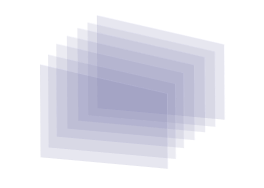
\includegraphics[scale=1]{1form.pdf}
\end{center}

The space of 1-forms is a vector space itself and considered the dual space to $\mathbb{R}^n$, denoted $(\mathbb{R}^n)^*$

Given a basis $(x_1,...,x_n)$ for some vector space $\Rn$ there is a natural corresponding basis for 1-forms denoted $(x^1,...,x^n)$. So any 1-form $\omega$ in $\Rn$ may be written 

\input{natdbasis.pdf_tex}

$$
\omega=\sum_n a^i x_i=a^i x_i=a^idx_i
$$

As a heuristic, dual vectors can be thought of as objects that eat vectors and return scalars from the underlying field in a linear way. sometimes offering a way to measure vectors?

\begin{center}
\input{1formvector.pdf_tex}
\end{center}

\textbf{Definition:} The \textit{cotangent space} $T^*_p\M$ at some point $p$ in manifold $\M$ is the dual space to the tangent space at $p$. 


\input{tstarpm.pdf_tex}

Elements of the cotangent space are denoted $df$, and are analagous to incremental changes of functions $f:\M\rightarrow\R$ via $df=\frac{\partial f}{\partial x^{\mu}}dx^{\mu}$. Elements of the tangent space are denoted $V$, and are analagous to directional derivatives $v^{\mu}\frac{d}{dx^{\mu}}$. Then, $df(V)$, is the directional derivative of $f$ in the direction of $V$, i.e. $df(V)=v^{\mu}\frac{df}{dx^{\mu}}$.

%\input{fdf.pdf_tex}


\textbf{Definition:} A tensor product space $U\otimes V$ between two vector spaces $ U,V $ is a space specially constructed such that bilinear maps of the form $g:U\times V\rightarrow\mathbb{F}$ correspond naturally to linear maps $\tilde{g}:U\otimes V\rightarrow\mathbb{F}$ out of the tensor product space.  
 
Now consider the tensor space characterized by $q,r$ via

$$
\mathfrak{T}^q_{r,p}(\M )= (\underbrace{ T_p\M\otimes T_p\M\otimes ... \otimes T_p\M }_q)\otimes (
\underbrace{T_p^*\M\otimes ...\otimes T^*_p\M }_r)
$$

where $T\in\mathfrak{T}^q_{r,p}(\M )$ is called a tensor of type $(q,r)$ and is a vector in the vector space $\mathfrak{T}^q_{r,p}(\M )$. A basis for $\mathfrak{T}^q_{r,p}(\M )$ can be constructed by taking the tensor product of all possible combinations of basis elements, $(x_{i_{1}}\otimes x_{i_{2}}\otimes ... \otimes x_{i_{q}})\otimes (x^{i_{1}}\otimes ... \otimes x^{i_{r}})$, where $1\leq i\leq dim(\M )$. Thus, elements $T\in\mathfrak{T}^q_{r,p}(\M )$ have the form 

$$
T=T^{i_1i_2..i_q}_{i_1..i_r}\frac{\partial}{\partial x^{i_1}}\otimes...\otimes\frac{\partial}{\partial x^{i_q}}\otimes dx^{i_1} \otimes ... \otimes dx^{i_r}
$$

and are linear functions on the space $\left(\bigotimes_{j=1}^{q}T^*_p\M \right) \otimes\left(  \bigotimes_{k=1}^{r}T_p\M\right)$.

\textbf{Definition:} A \textit{vector field} is a map $\M\rightarrow T_p\M$ that assigns a vector to each point in $p\in\M$ smoothly. The set of vector fields on a manifold $\M$ will be denoted $\mathcal{X}(\M)$

\textbf{Definition:} A \textit{tensor field} is a map $\M \rightarrow \mathfrak{T}^q_{r,p}(\M )$ that smoothly assigns each point $p\in\M$ a tensor of type $(q,r)$. The set of tensor fields on a manifold $\M$ will be denoted $\mathfrak{T}^q_{r}$.

Notice $\mathfrak{T}^0_0=\mathcal{F}(\M)$ and $\mathfrak{T}^1_0=\mathcal{X}(\M)$.
  

\textbf{Note:} Given some tensor space $V\otimes V\otimes...\otimes V$, there are two natural subspaces.

The \textit{symmetric group} on $\underbrace{\otimes ... \otimes V}_n$ with the action $S_n$ given by 

$$
S_n=\lbrace x\in S_n \iff x\in \pi (1,2,...,n)\rbrace
$$

Where $\pi (1,2,...,n):V\otimes ... \otimes V \rightarrow V\otimes ... \otimes V$ is a permutation on $V\otimes ... \otimes V$ via $\pi (V_1\otimes ... \otimes V_n )=V_{\pi (1)}\otimes ... \otimes V_{\pi (n)}$. $S_n$ then gives a way to define a symmetric subspace $Sym_n(V)$ and an anti-symmetric subspace $\bigwedge^n(V)$ as

$$
Sym_n (V) \equiv \lbrace v \vert \pi (v)=v \ \ \ \forall \pi \in S_n\rbrace
$$

$$
\bigwedge^n(V)\equiv \lbrace v\vert \pi (v)= sgn(\pi ) v\rbrace
$$
 
 \begin{center}
 where $sgn(\pi)$ is defined as $(-1)^{\# \ of \ transpositions \ of \ \pi}$  
\end{center}  
 
$k$-forms can then be thought of as the anti-symmetric subspace of the tensor product of some cotangent space with itself $k$ times
 
 
 \textbf{Definition} An \textit{exterior form of degree} $k$, or $k$-form, $\omega$  is a $k$-linear anti-symmetric function of $k$ vectors. Formally,
 
 $$
 \omega (\alpha \chi_1 + \beta \nu_1,\xi_2,...\xi_k )=\alpha \omega (\chi_1,\xi_2,...\xi_k )+\beta \omega (\nu_1,\xi_2,...\xi_k )
 $$
 
\begin{center}

\end{center} 
 
$$
\omega(\chi_{\pi(1)},...,\chi_{\pi(k)})=sgn(\pi) \omega(\chi_1,...,\chi_n)
$$ 
 
Alternatively, $\omega\in\bigwedge^k(V^*)$. Note that $\bigwedge^k(V)=P_-(V\otimes...\otimes V)\equiv \frac{1}{k!}\sum_{\pi\in S_n}V_{\pi}\otimes ... \otimes V_{\pi}$. In consideration of $k$-forms there is a natural product to define, namely the exterior product or anti-symmetric product 
 (or wedge product).
 
\textbf{Definition:} The \textit{exterior product} $\omega_k\wedge \omega_l$, where $\omega_k$ is a $k$-form and $\omega_l$ is an $l$-form, is a $(k+l)$-form such that 

$$
\omega_k\wedge\omega_l=(-1)^l \omega_l\wedge\omega_k
$$
 
and actions of $\omega_k\wedge \omega_l$ on a vector $v_1\otimes ... \otimes v_{k+l}\in V^{\otimes(k+l)}$ is given by 

$$
(\omega_k\wedge \omega_l)(v_1\otimes ... \otimes v_{k+l})=\frac{1}{k!}\frac{1}{l!}\sum_
{\pi\in S_{(k+l)}}sgn(\pi )\omega^k(v_{\pi(1)}\otimes ... \otimes v_{\pi(k)})\omega^l(v_{\pi(k+1)}\otimes ... \otimes v_{\pi(k+l)})
$$  
 
and 

$$ 
 (\omega^k\wedge\omega^l)\propto P^{(k+l)}_{-}(\omega^k\otimes\omega )
$$
 
A basis for $\bigwedge^{k}(V)\equiv \underbrace{ V\wedge ...\wedge V}_k$ given a basis $e
 _j$ for $V$ is constructed by

$$
e_{j_1}\wedge e_{j_2}\wedge... \wedge e_{j_k}; \ \ \ j_1 < j_2<...<j_k
$$

As $e_j\wedge e_j=0$ and the operation is antisymmetric so any rearrangement of the same basis elements is at most changed by a negative phase


For any smooth function $f:\M\rightarrow\mathcal{N}$ from one manifold to another, there is an induced map on the respective tangent spaces, $df:T\M\rightarrow T\mathcal{N}$.

\begin{center}

\input{inducedmap.pdf_tex}

\end{center}

\textbf{Definition:} A manifold $\M$ with some atlas $\mathcal{A}$ is defined to be \textit{orientable} iff for any coordinate basis $x^n$ for $U_x \in\mathcal{A}$ and $y^n$ for $U_y \in\mathcal{A}$ covering $\M$ we have

$$
J=det\left( \frac{\partial x^n}{\partial y^k} \right)>0
$$ 
 
 
If an $m$-dimensional manifold $\M$ is orientable there exists some $m$-form called a \textit{Volume Form} that is nonvanishing  
 
\pagebreak



\subsection{Problem Set 1}


1. (i) A torus is a manifold as it is locally euclidean at every point

(ii) A figure 8 is not a manifold as it intersects itself and at that point is not locally euclidean 

(iii) The manifold defined by $z-x^2-y^2=0$ requires atleast two charts in $\mathbb{R}^2$

(iv) The real projective space $\mathbb{R}P^n$ is the set of all lines passing through the origin in $\mathbb{R}^{n+1}$. Two points $\vec{x},\vec{y}\in\mathbb{R}^{n+1}$, define the same line if $\vec{x}=\alpha\vec{y}$ where $\alpha,\vec{x},\vec{y}\neq 0$. This gives us freedom to choose any point along each line as the representative for that line. 

Define $U_i$ to be the set of lines with $x_i\neq 0 \ (1\leq i\leq n+1)$. Now define charts $\phi_i:U_i\rightarrow \mathbb{R}^n$:

$$
\phi_i: (x_1,...,x_{n+1})\rightarrow \left(\frac{x_1}{x_i},...,\frac{x_{i-1}}{x_i},\frac{x_{i+1}}{x_i},...,\frac{x_{n+1}}{x_i}\right)
$$ 

For $\vec{x}\in U_i\cap U_j$, $\phi_j\circ\phi_i^{-1}=
\left(\frac{i_1 x_i}{x_j},...,\frac{x_i}{x_j} ,...,\frac{i_{j-1}x_i}{x_j},\frac{i_{j+1}x_i}{x_j},...,\frac{i_{n+1}x_i}{x_j}\right)
$

For $n+1=2$, $\vec{x}\in U_1\cap U_2$, $\phi_a\circ\phi_b^{-1}=
\left(\frac{bx_1}{x_2}\right) 
$ where $b$ is the input coordinate to the transition map and $\phi_a,\phi_b$ corresponds to $x_1,x_2$ respectively. This map is continuous as $x_1,x_2$ should never be zero according to the definition of the charts.

2. (i) Given the circle $S^1$ embedded in $\mathbb{R}^2$ via $x^2+y^2=1$ and the charts $\phi_1 ,\phi_2$:

$$
\phi_1^{-1}: (0,2\pi )\rightarrow S^1
$$

\vspace{-.3cm}

$$
\phi_1^{-1}: \theta \rightarrow (cos(\theta ),sin(\theta ))
$$

\medskip

$$
\phi_2^{-1}: (-\pi ,\pi )\rightarrow S^1
$$

\vspace{-.3cm}

$$
\phi_2^{-1}: \theta \rightarrow (cos(\theta ),sin(\theta ))
$$

It is easily seen that the charts overlap only in $(0,\pi )$, and thus $\phi_1\circ\phi_2^{-1}$ is defined in this range as $\theta_{\phi_2}\rightarrow\theta_{\phi_2}+\pi$

(ii) Given $S^2$ embedded in $\mathbb{R}^3$ via $x^2+y^2+z^2=1$, stereographic projection onto a plane under the sphere provides the chart

 $$\phi_s:S^2\rightarrow \mathbb{R}^2$$

 $$\phi_s:(x,y,z)\rightarrow (X=\frac{x}{1-z},Y=\frac{y}{1-z})
 $$
 
Which is well defined everywhere except for $z=1$, and thus atleast one more chart is required.

(iii) Polar coordinates also provide a chart $\psi:S^2\rightarrow \mathbb{R}^2$ for the sphere given by 

$$
\psi^{-1}: (\theta ,\phi)\rightarrow(x=sin\theta cos\phi\,\ y=sin\theta sin\phi, \ z=cos\theta)
$$

which also fails for one point, $\theta=0$. Composition of the inverse map of polar coordinates and stereographic projection then yields

$$
\phi_s\circ\psi^{-1} :(\theta,\phi)\rightarrow (X=\frac{sin\theta cos\phi}{1-cos\theta},Y=\frac{sin\theta sin\phi}{1-cos\theta})
$$

3. (i)Vectors are directional derivatives, scalars are real numbers. Easily seen to satisfy distributivity, associativity rules satisfied as it would be for functions.

(ii)$X[x^i(t)]$ can be interpreted as velocity in the $x^i$ direction at time $t$

\pagebreak

\subsection{Problem Set 2}

1. (i) See E-L derivation section. % Note that $\frac{\partial L}{\partial q}=\frac{\partial L}{\partial x}\frac{\partial x}{\partial t}$ think

(ii) Given $L=\frac{1}{2}g_{ij}(x_{\nu})\dot{x}^i\dot{x}^j$ where $g_{ij}$ is given to be a function of position, symmetric in $i,j$ and $g^{ik}g_{kj}=\delta^i_j$

Applying EL eq.,

$$
\frac{d}{dt}\frac{d}{d\dot{x}^{\alpha}}\left(
\frac{1}{2}g_{ij}(x_{\nu})\dot{x}^i\dot{x}^j
\right)=\frac{d}{dx^{\alpha}}\left(
\frac{1}{2}g_{ij}(x_{\nu})\dot{x}^i\dot{x}^j
\right)
$$


$$
\frac{d}{dt}\frac{d}{d\dot{x}^{\alpha}}\left(
\frac{1}{2}g_{ij}(x_{\nu})\dot{x}^i\dot{x}^j
\right)= \frac{d}{dt}\left( \frac{1}{2}g_{ij}(\delta^{\alpha}_{i}\dot{x^j}+\dot{x^i}\delta^{\alpha}_{j})\right)=\frac{d}{dt}\left( g_{\alpha j}\dot{x^j}\right)=g_{\alpha j}\ddot{x}^j
$$

$$
\frac{d}{dx^{\alpha}}\left(
\frac{1}{2}g_{ij}\dot{x}^i\dot{x}^j
\right)
$$


2. (i.) Given $n$ different 1-forms $\omega_i$ and a permutation $\pi$ of $\lbrace 1,...,n\rbrace$, show that 

$$
\pi(\omega_1\wedge ... \wedge \omega_n)= sgn(\pi)\omega_1\wedge...\wedge\omega_n
$$

Given the wedge product is antisymmetric and the fact that permutations are partitioned by requiring an odd or an even number of transpositions, it follows that the required rearrangement to achieve $\pi$ is equal to $(-1)^{0\ if\ even \ or\ 1\ if \ odd}$.



(ii.) Prove that the dimension of the vector space $\bigwedge^k V$ is 
$\begin{bmatrix}
n \\
k
\end{bmatrix}
$.
For a $k$-form in $n$ dimensions, there are $\frac{n!}{(n-k)!}$ choices of orders of basis vectors but due to anti-symmetry,   
there are $k!$ rearrangements of any $k$-form up to some negative phase and $\frac{n!}{(n-k)!k!}=nCk$. As such, the dimension of $\bigwedge^n V=1$.

(iii.) 3-forms in the space of $\R^3$ take the form:

$$
f(x,y,z)dx\wedge dy\wedge dz
$$

This manifold should be orientable? Jacobian always positive/unital?

3. (i.) on arch

(ii.) 1-forms on $\R$ will have the form $\omega=f(x)dx$ which is clearly closed and exact as some function can be defined $\frac{dg}{dx}=f,\ g=\int f(x) dx$.

(iii.) Given the following form in $\R^2$, 

$$
\omega=\frac{-y}{x^2+y^2}dx + \frac{x}{x^2+y^2}dy
$$

calculate $d\omega$.

$$
d\omega=\left(\frac{d}{dy}\frac{y}{x^2+y^2}+\frac{d}{dx}\frac{x}{x^2+y^2}\right) dx\wedge dy=\left(\frac{1}{x^2+y^2}+\frac{-y}{(x^2+y^2)^2}(2y)+\frac{1}{x^2+y^2}+\frac{-x}{(x^2+y^2)^2}(2x)\right) dx\wedge dy
$$

$$
=0
$$

We know $\omega\neq df$ for any function $f(x,y)$ and thus is not exact as this would entail 

$$
\frac{\partial f}{\partial x}=\frac{-y}{x^2+y^2},\ \frac{\partial f}{\partial y}=\frac{x}{x^2+y^2}
$$

but for a function we should have $\frac{\partial }{\partial y}\frac{\partial f}{\partial x}=\frac{\partial }{\partial x}\frac{\partial f}{\partial y}$, which is clearly not satisfied here as

$$
\frac{\partial }{\partial y}\frac{\partial f}{\partial x}=\frac{\partial }{\partial y}\frac{-y}{x^2+y^2}=\frac{1}{x^2+y^2}+\frac{-y}{(x^2+y^2)^2}(2y)
$$

$$
\frac{\partial }{\partial x}\frac{\partial f}{\partial y}=\frac{\partial }{\partial x}\frac{x}{x^2+y^2}=\frac{1}{x^2+y^2}+\frac{x}{(x^2+y^2)^2}(2x)
$$

\begin{sympycode}
x, y, z =symbols('x y z')
\end{sympycode}

$\sympy{simplify(diff(-y/(x**2+y**2),y)+diff(-x/(x**2+y**2),x))}$


\begin{sympycode}
myvar = 125
\end{sympycode}

$\sympy{myvar}$

\subsection{Problem Set 3}


1. (i) show that this atlas for the Mobius strip  is not orientable: charts $(x^1,x^2)$ and $(y^1,y^2)$ that overlap in regions $A_1$ of chart $x$ and $A_2$ of chart $y$ with transition map $x^1=y^1+7$, $x^2=y^2$ and overlap in regions $B_1$ of chart $x$ and $B_2$ of chart $y$ with transition map $x^1=y^1-7$, $x^2=-y^2$.

(ii) Explain why all one-dimensional manifolds are orientable: A one dimensional manifold will always have charts of the form $x^i$ where there is only one parameter $x$ for every chart $i$. Thus $J=\frac{\partial x^i}{\partial x^j}$





lecture 4 1:05:00 for ex statement

lecture 5 1:09:00

lecure 5 1:23:00

%\cite{arnold1989}

%\cite{coopersmith2017}

\bibliography{try.bib}{}
\bibliographystyle{plain}


\end{document}
